%
% -----------------------------------------------------------------------------
\section{Model description}
The model used for this demo corresponds to the model proposed by 
\citet{midzi1999} in the context of the GSHAP project.
As illustrated in Figure \ref{fig:ssa_area_sources}, this 
seismic source model contains 21 area sources distributed along a wide 
band ideally connecting from the Red Sea with South Africa.

The area sources part of this model can be ideally subdivided into a small 
number of groups.
To the north, a first class of area sources cover the three branches 
of the triple junction in the Afar region. 
The following set of sources shows a spatial pattern that reproduces
the structural trend of the graben systems composing the two main 
branches composing the continental part of the East African Rift:
the Western and East branches. The last set of sources includes the 
southermost part of the model where rift's textonic structure are less
evident and the seismicity spreads over a wide sectors (see Figure
\ref{fig:Subsahara_Catalogue_ISC_1}).
%
\begin{figure}[ht]
	\centering
	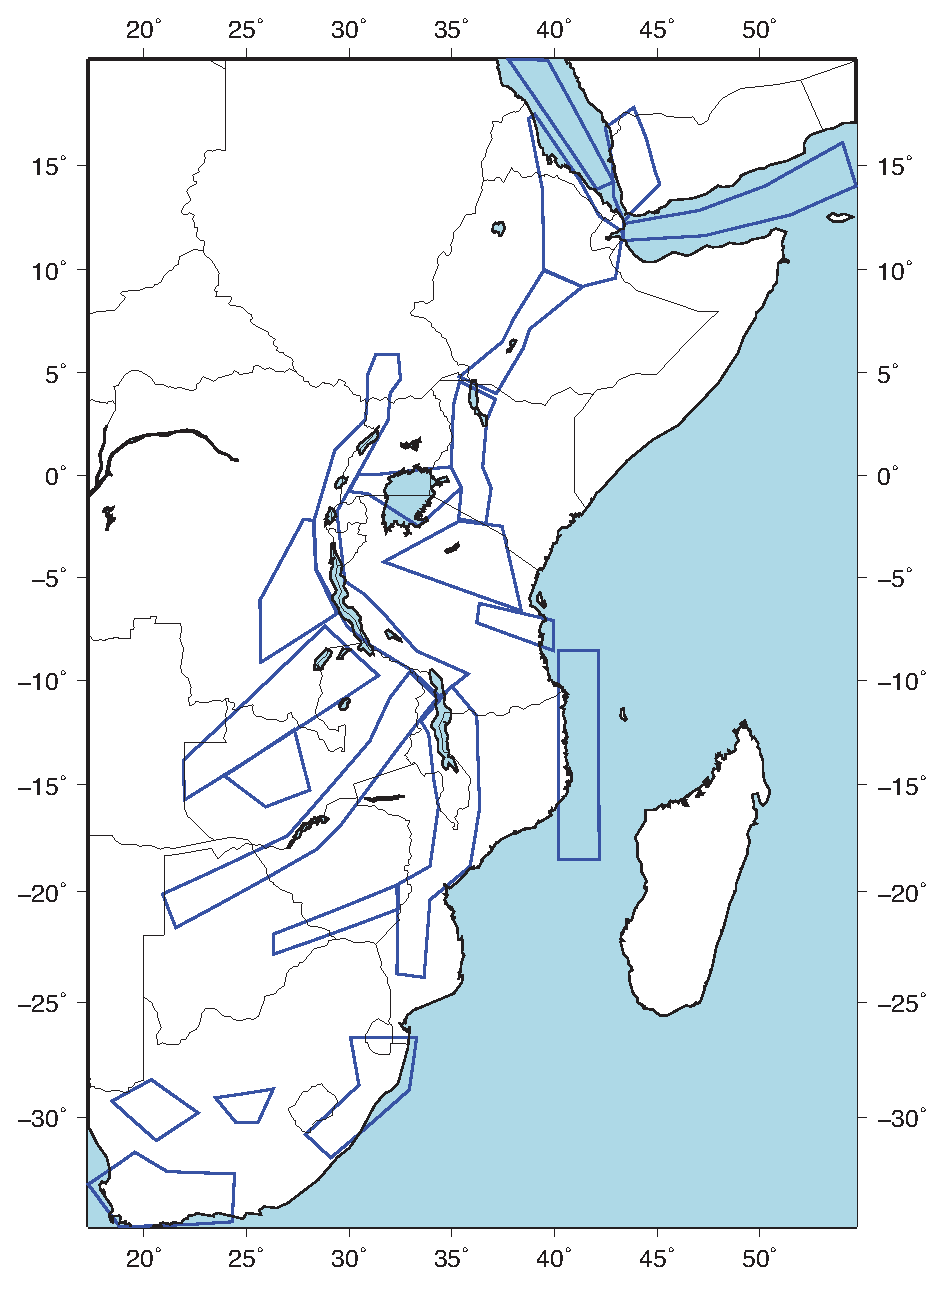
\includegraphics[width=10cm]
        {./figures/ssa_area_sources.eps}
	\caption{Area sources in the demo PSHA input model.}
	\label{fig:ssa_area_sources}
\end{figure}
%
The seismicity recurrence parameters and the maximum magnitude 
assigned to the different sources corresponds to the ones originally
determined by \citet{midzi1999}.

The maximum magnitude ranges between 6.5 and 7.8; the sources with the
highest potential 

The 

%
% -----------------------------------------------------------------------------
\section{Assignment: hazard calculation using the demo model}
The first assignment focuses on the calculation of hazard for a small area 
using Openquake and demo model provided.


\clearpage
%
% -----------------------------------------------------------------------------
\subsection{Analysis of results}













\section{A brief demo of the Modeller's Toolkit - An African example}
The following will outline how to use the Modeller's Toolkit for the above 
example. In this exercise we shall be using the GSHAP area sources used in 
the previous demonstration, and utilising a new earthquake catalogue to 
recalculate the activity rates for the zones. This same process could be 
applied to any earthquake catalogue for the region and any area source 
zone model. 

\subsection{The Earthquake Catalogues}

Two earthquake catalogues are used for this exercise:
\begin{enumerate}
\item The Global CMT database (1976 - 2011) (Figure 
    \ref{fig:Subsahara_Catalogue_GCMT_1})
\item A ''Homogenised'' Instrumental Catalogue - Derived from the ISC 
    bulletin, converting the magnitudes from different agencies 
    according to a hierarchical selection (Figure 
    \ref{fig:Subsahara_Catalogue_ISC_1})
\end{enumerate}
\textbf{The ''Homogenised'' Catalogue has been created only for the 
purposes of the demonstration. There is NO ASSURANCE OF QUALITY and 
therefore the catalogue should NOT be used for any other purposes 
than demonstration!}

\begin{figure}[htbp]
	\centering
		\includegraphics[height=16cm, keepaspectratio=true]{./figures/Subsahara_Catalogue_GCMT_1.eps}
	\caption{Sub-Saharan Catalogue - GCMT}
	\label{fig:Subsahara_Catalogue_GCMT_1}
\end{figure}

\begin{figure}[htbp]
	\centering
		\includegraphics[height=16cm, keepaspectratio=true]{./figures/Subsahara_Catalogue_ISC_1.eps}
	\caption{Sub-Saharan Catalogue - ''New Homogenised''}
	\label{fig:Subsahara_Catalogue_ISC_1}
\end{figure}


\cleardoublepage
